% !Mode:: "TeX:UTF-8"
\chapter{代码实现}

我选择使用python实现RSA算法,因为python原生提供了对高精度数字的支持,便于实现。

代码链接放在了附录\ref{chapter-faq}中。

运行结果如下:
% 添加图片

\begin{figure}[htbp]
    \centering
    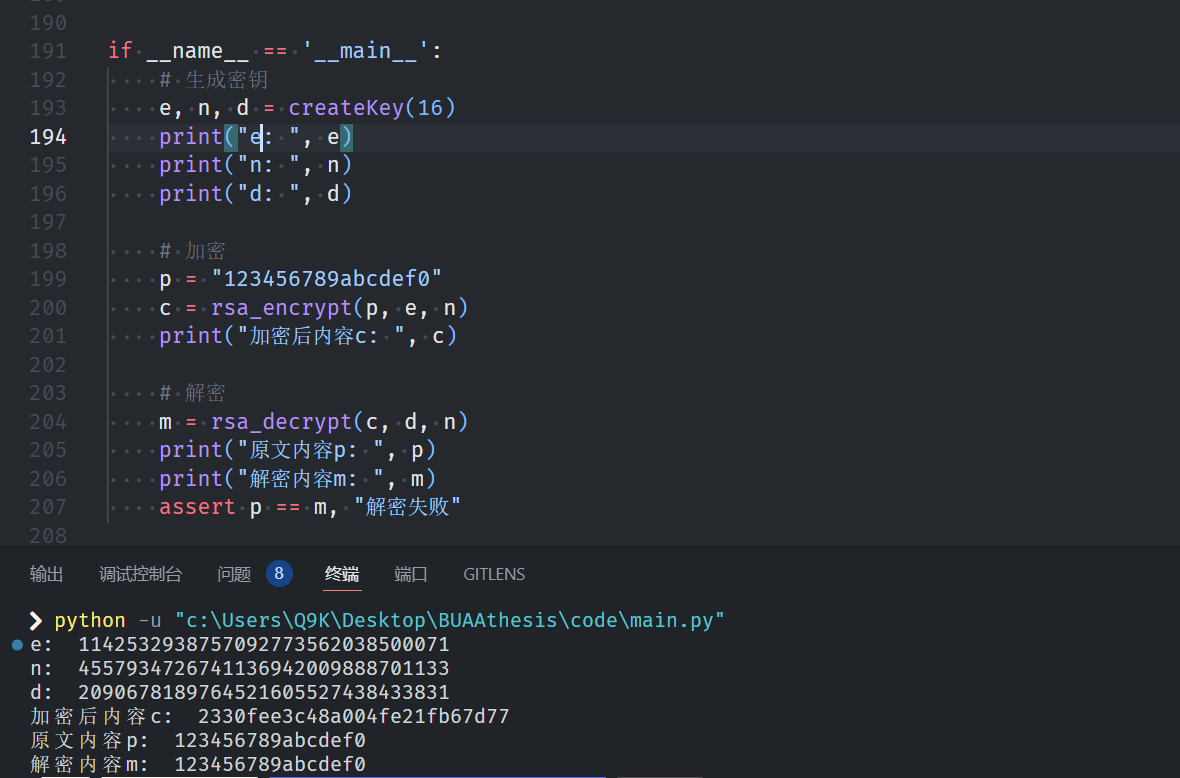
\includegraphics[scale=0.8]{data/image/code_result.jpg}
    \caption{代码运行结果}
    \label{figure1}
\end{figure}